\part{Was ist KI?}
\chapterimage{Bilder_und_Co/a_magnifying_glass_which_points_out_a_neuronal_network_surrounded_by_computer_code_and_a_question_ma_296098326.png} % Chapter heading image
%----------------------------------------------------------------------------------------
\chapter{Definition und Einordnung}
In diesem Kapitel wir erklärt was \ac{KI} ist, 
wie verschiedene Dinge einzuordnen sind 
und weitere wichtige Begrifflichkeiten geklärt, 
die zu einem tieferen Verständnis für das Thema wichtig sind.

\section{Definition}
Als \ac{KI} bezeichnet man die Fähigkeit einer Maschine bzw. eines Computers, 
die die Fähigkeiten von Menschen übertrifft.

(Zu beachten gilt, dass sich das 
unteranderem auf nieschen Bereiche beziehen kann. Z.B. wenn die Temperaturanzeige 
einen gewissen Wert übschreitet einen Knopf zu drücken für die Zusatzkühlung. Hier 
übertrifft die Maschine die Konzentrationsfähigkeit eines Menschen. Diese einfache 
Automatisierung fällt bereits unter die Begriflichkeit von KI, was das Thema 
relativ unintuitiv macht. Meistens bezieht man sich im Alltag auf DNNs, z.B. 
ChatGPT.)

\section{Einordnung}
Man kann \ac{KI} in sieben Kategorien unterteilen, 
davon beschreiben drei die Überkategorien:
\smallskip
\begin{itemize}
    \item \textbf{Narrow \ac{AI}}
    
    Oft auch als schwache KI bezeichnet, ist die einzige Form von KI, 
    die bisher existiert. Narrow \ac{AI} übertrifft die Fähigkeiten von Menschen
    in sehr begrenzten Aufgaben und bedarf außerhalb dieser die Hilfen von Menschen.
    Narrow \ac{AI} lässt sich in zwei Unterkategorien unterteilen:
    
    \subitem \textbf{Reactive Machines}

    Diese übertreffen den Menschen meist auf Grund ihrer Ausdauer, 
    da diese Einschränkungen wie Aufmerksamkeitspannen nicht besitzen. 
    Zudem treffen Reactive Machines Entscheidungen nur anhand von zu diesem Zeitpunkt bestehenden Informationen.
    Ein Bespiel hierfür ist das bekannte Schachspiel Programm von IBM.
    
    \subitem \textbf{Limited Memory}

    Limited Memory \ac{AI} hingegen trifft Entscheidungen anhand von gesammelten Daten, 
    ähnlich zu einem Kurzzeitgedächtnis. Die Begrenztheit, wie es aus dem Namen hervorgeht, 
    kommt daher, dass diese \ac{KI} kein Langzeitgedächtnis besitzt und daher die Daten nicht über längere Zeit speichern kann. 
    Beispiele hierfür sind Chatbots wie ChatGPT oder autonome Fahrzeuge.
    
    \item \textbf{\ac{AGI}}
    
    Oder auch Starke \ac{KI} genannt, ist lediglich theoretisch definiert und existiert noch nicht. 
    \ac{AGI} besitzt nur eine Unterkategorie: \textbf{Theory of Mind}. 
    Wie bereits zuvor besschreibt diese ebenfalls die Fähigkeiten einer solchen \ac{KI}. 
    Thery of Mind ist definiert, dass sie zuvor Gelerntes und erhaltene Fähigkeiten, 
    ohne weiteres zutun von Menschen das Model auf diese zu trainieren einsetzen kann.
    
    \item \textbf{\ac{ASI}}
    
    Existiert ebenfalls nur auf theoretischer Basis und wird als \textbf{Self Aware} \ac{KI} bezeichnet. 
    \ac{ASI} soll denken, kombinieren und lernen können, sowie kognitive Fähigkeiten besitzen, 
    die die Fähigkeiten von Menschen übersteigen soll.
\end{itemize}

\section{Begriffe}
Im Folgenden Schaubild sind welche der wichtigsten Begriffe da gestellt und ihre Beziehung zueinander. 
Z.B. ist Deep Learning Teil von Maschinellen Lernen. Dieses dient zum einfachen und schnellen visuellen Einordnen. 
Zum Thema dieser Arbeit sind zu folgenden Kontexten Begriffe wichtig:
\smallskip
\begin{itemize}
    \item \textbf{Radar-Rohdaten}
        Zur Bilderkennung oder Verarbeitung von Radar-Rohdaten sind Vision Transformer bzw. Vision Models 
        derzeit von großer Bedeutung.

    \item \textbf{Radar Daten}
        Um Muster in Radar Daten sichtbar zu machen wird in verschiedenen Papern Custering verwendet. 
        Meist nachdem die Rohdaten bereits mittels Fast Fourier Transformation aufbereitet wurden.
        
    \item \textbf{Schemata}
        Um innerhalb großer Datenmengen Schemata zu visualisieren und erste Zusammenhänge zu erkennen, 
        werden oft Decision Trees verwendet. Gerade der Wissenschaftliche Bereich Datascience setzt sich 
        damit auseinander anhand großer Mengen von Daten Muster zu erkennen. Maschinelles Lernen 
        bzw. KI sind von den dort verwendeten Werkzeugen die wertvollsten. 

\end{itemize}

\begin{figure}[h]
\centering
\vspace{1cm}

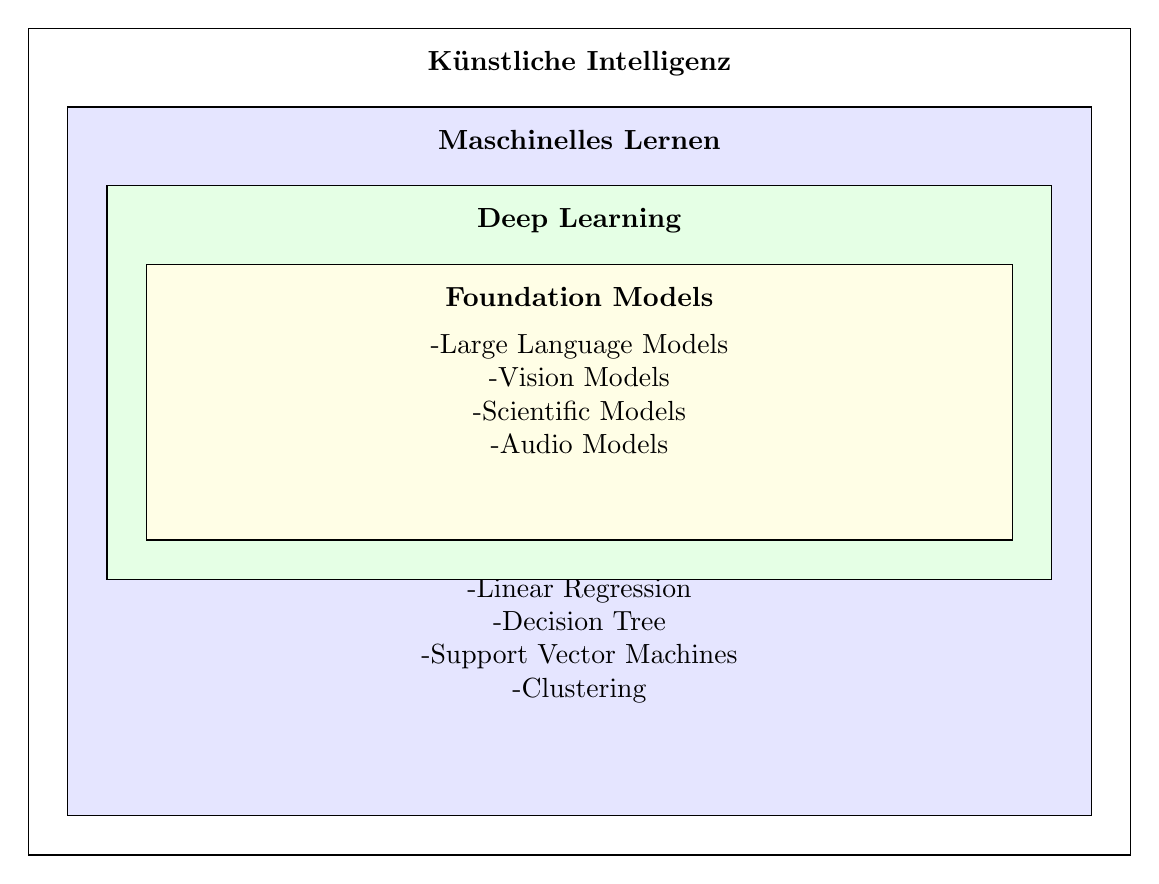
\begin{tikzpicture}
    % Oberster Punkt für das äußerste Rechteck
    \coordinate (topA) at (0,0);

    % Äußeres Rechteck
    \node[draw, minimum width=14cm, minimum height=10.5cm, anchor=north] (A) at (topA) {};
    \node[anchor=north, align=center] at (A.north) [yshift=-5pt] {\textbf{Künstliche Intelligenz}};

    % 2. Rechteck: oberer Rand etwas unter A.north
    \coordinate (topB) at ([yshift=-1cm]A.north);
    \node[draw, fill=blue!10, minimum width=13cm, minimum height=9cm, anchor=north] (B) at (topB) {};
    \node[anchor=north, align=center] at (B.north) [yshift=-5pt] 
        {\textbf{Maschinelles Lernen}
        \\[15em]-Linear Regression
        \\-Decision Tree
        \\-Support Vector Machines
        \\-Clustering
        };

    % 3. Rechteck: oberer Rand etwas unter B.north
    \coordinate (topC) at ([yshift=-1cm]B.north);
    \node[draw, fill=green!10, minimum width=12cm, minimum height=5cm, anchor=north] (C) at (topC) {};
    \node[anchor=north, align=center] at (C.north) [yshift=-5pt] {\textbf{Deep Learning}};

    % 4. Rechteck: oberer Rand etwas unter C.north
    \coordinate (topD) at ([yshift=-1cm]C.north);
    \node[draw, fill=yellow!10, minimum width=11cm, minimum height=3.5cm, anchor=north] (D) at (topD) {};
    \node[anchor=north, align=center] at (D.north) [yshift=-5pt] 
        {\textbf{Foundation Models}
        \\[0.5em]-Large Language Models
        \\-Vision Models
        \\-Scientific Models
        \\-Audio Models
        };
\end{tikzpicture}

\caption{Verschachtelte Begriffe}
\end{figure}

\chapter{KI im Einsatz}
\section{KI im Alltag}
Einige Beispiele in alltäglichen Situationen, in denen man auf KI trifft. Manche Beispiele dienen dazu sich 
Bewusst zu werden wie, wo und wie oft man Kontakt zu KIs hat. Andere Beispiele dienen zur Veranschaulichung, 
wie Personen oder Branchen mit KIs umgehen, auf die Luftfahrt übertragen werden können oder bereits stattfinden:
\smallskip
\begin{itemize}
    \item \textbf{Kommunikation allgemien}
        Aus verschiedenen Erfahrungsberichten, sowohl aus persöhnlichem Umfeld als auch durch Medien 
        vermitteltes Allgemeinwissen, werden z.B. Chatbots wie ChatGPT verwendet um Emails zu beantworten.
        Um alltägliche Aufgaben wie Emails zu beantworten, sowohl im privaten als auch im Geschäft gehört 
        es inzwischen zum Alltag diese Aufgabe zumindest teilweise zu automatisieren. Hier werden meist die 
        von der KI verfassten Emails nur noch gegen gelesen und gegebenenfalls korrigiert, da diese Methode 
        Zeit spart und weiter eine konsistente professionelle Sprache zu gewährleisten.

    \item \textbf{Kommunikation auf verschiedenen Sprachen}
        Bei internationaler Kommunikation bleibt es nicht aus, sich auf einer anderen Sprache wie die eigenene 
        Muttersprache zu unterhalten. Teil davon ist es, einzelne Begriffe nachzuschlagen oder ganze Texte zu 
        übersetzen. Bereits um einzelne Begriffe nachzuschlagen wird fast ausschließlich Übersetzungssoftware 
        Benutzt, da das Nachschlagen in einem Buch zu Zeitaufwändig ist. Da inzwischen inzwischen die gängigsten 
        Übersetzungssoftware wie Google Translater und DeepL ebenfalls KI verwenden ist der Kontakt oder die 
        Verwendung von KI nahezu unvermeidbar.
        
    \item \textbf{Recherche}
        Ein weiteres alltägliches Bespiel ist die Google Recherche. Auch hier ist bei jeder Google Suche 
        standarmäßig eine KI im Einsatz, die durch kurzes Zusammenfassen der wichtigsten Abschnitte der 
        wichtigsten Websites im Bezug zum Suchbegriff das nachschlagen erleichtert. Zudem gibt die KI Vorschläge 
        zu verwanten Begriffen, Fragen oder anderen Google Suchen um die Nutzererfahrung zu verbessern. 
                
    \item \textbf{Arbeiten im Büro}
        Microsoft Copilot ist eine KI, die standardmäßig bei alltäglichen Programmen wie Word und Excel 
        eingebunden ist. Diese zwei genannten Programme sind welche der weitverbreitetsten und in 
        verschiedenen Branchen welche der Essentiellsten Programme. Hier unterstützt KI die Rechtschreibung, 
        den Satzbau und das automatische Erkennen und Erstellen von Formeln.

    \item \textbf{Passiv}
        Oft ist man sich nicht Bewusst, dass eine KI verwendet wird. Ein Beispiel hierfür ist ein Email Spamfilter, 
        diese Filter haben teilweise eine KI, die die Emails auf Schlüsselwörter untersucht mit dabei.
        Weitere Beispiele, die KI verwenden sind: die Schildererkennung in modernen Fahrzeugen oder Trend 
        und Recommendation Algorithmen auf Social Media wie Youtube oder X.

    \item \textbf{Indirekt}
        In der Forschung in z.B. der Medizin oder Materialforschung wird KI verwendet um Eigenschaften vorher 
        sagen zu können von neuen Zusammensetzungen bekannter Stoffe. Diese neu gefundenen Medikamente oder 
        Legierungen können nach ausreichenden Tests verwendet werden.

\end{itemize}

\section{Zusammenfassung}
Anhand dieser alltäglichen Beispiele sowohl in der Technik als auch im Alltag von den Meisten 
Personen in nahezu jeder Technik, Logistik und vielen weiteren Branchen sollte klar geworden sein, dass 
der Einsatz von KI im Jahr 2025 unvermeidbar geworden ist, egal ob aktiv oder passiv bzw. bewusst oder unbewusst. 
Darüber hinaus kann man sagen, dass zumindest eine Art schleichende Adaptierung stattfindet. 
Daher sollte man sich zeitnahe Gedanken machen, wie man mit dieser Technologie umgehen sollte. 
In dieser Arbeit im Hinblick auf Sicherheit.